\section{Algebraic polyhedra}\label{Algebraic}

Normaliz can use coefficients from real algebraic extensions of $\QQ$. It is clear that the computations are then restricted to those that do not depend on finite generation of monoids. Whether algebraic coordinates are needed, is decided when Normaliz reads the input file and checks whether it defines an algebraic extension of $\QQ$ embedded into $\RR$.

\subsection{An example}\label{alg_ex}

The icosahedron, one of the platonic solids, needs $\sqrt 5$ for its coordinates. Via its vertices it can be defined as follows (\verb|icosahedron-v.in|, picture by J.-Ph.~Labbé):

\begin{minipage}[b]{0.5\textwidth}
	\begin{verbatim}
	
	amb_space 3
	number_field min_poly (a^2 - 5) embedding [2 +/- 1]
	vertices 12
	0 2 (a + 1) 4
	0 -2 (a + 1) 4
	2 (a + 1) 0 4
	...
	(-a - 1) 0 -2 4
	Volume
	ModuleGenerators
	FVector
	EuclideanAutomorphisms
	
	\end{verbatim}
\end{minipage}
\hspace{1.5cm}
\begin{minipage}[t]{0.4\textwidth}
	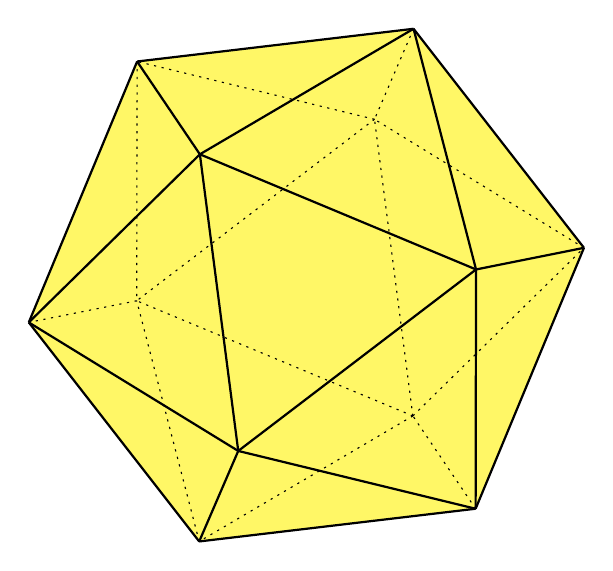
\begin{tikzpicture}%
	[x={(0.700041cm, -0.429565cm)},
	y={(0.714101cm, 0.419519cm)},
	z={(0.001418cm, 0.799673cm)},
	scale=3.800000,
	back/.style={dotted, thin},
	edge/.style={color=black!95!black, thick},
	facet/.style={fill=yellow,fill opacity=0.600000},
	vertex/.style={inner sep=0pt,circle,draw=black!25!black,fill=black!75!black,thick}]
	%
	%
	%% Coordinate of the vertices:
	%%
	\coordinate (0.80902, 0.00000, 0.50000) at (0.80902, 0.00000, 0.50000);
	\coordinate (0.80902, 0.00000, -0.50000) at (0.80902, 0.00000, -0.50000);
	\coordinate (0.00000, 0.50000, 0.80902) at (0.00000, 0.50000, 0.80902);
	\coordinate (0.00000, 0.50000, -0.80902) at (0.00000, 0.50000, -0.80902);
	\coordinate (0.50000, 0.80902, 0.00000) at (0.50000, 0.80902, 0.00000);
	\coordinate (-0.50000, 0.80902, 0.00000) at (-0.50000, 0.80902, 0.00000);
	\coordinate (0.00000, -0.50000, 0.80902) at (0.00000, -0.50000, 0.80902);
	\coordinate (0.00000, -0.50000, -0.80902) at (0.00000, -0.50000, -0.80902);
	\coordinate (0.50000, -0.80902, 0.00000) at (0.50000, -0.80902, 0.00000);
	\coordinate (-0.80902, 0.00000, 0.50000) at (-0.80902, 0.00000, 0.50000);
	\coordinate (-0.80902, 0.00000, -0.50000) at (-0.80902, 0.00000, -0.50000);
	\coordinate (-0.50000, -0.80902, 0.00000) at (-0.50000, -0.80902, 0.00000);
	%%
	%%
	%%
	%%
	%% Drawing vertices in the back
	%%
	% \node[vertex] at (0.00000, 0.50000, -0.80902)     {};
	% \node[vertex] at (-0.80902, 0.00000, -0.50000)     {};
	% \node[vertex] at (-0.50000, 0.80902, 0.00000)     {};
	%%
	%%
	%% Drawing the facets
	%%
	\fill[facet] (0.00000, -0.50000, 0.80902) -- (0.80902, 0.00000, 0.50000) -- (0.00000, 0.50000, 0.80902) -- cycle {};
	\fill[facet] (-0.80902, 0.00000, 0.50000) -- (0.00000, 0.50000, 0.80902) -- (0.00000, -0.50000, 0.80902) -- cycle {};
	\fill[facet] (0.50000, 0.80902, 0.00000) -- (0.80902, 0.00000, 0.50000) -- (0.00000, 0.50000, 0.80902) -- cycle {};
	\fill[facet] (0.50000, 0.80902, 0.00000) -- (0.80902, 0.00000, 0.50000) -- (0.80902, 0.00000, -0.50000) -- cycle {};
	\fill[facet] (0.50000, -0.80902, 0.00000) -- (0.80902, 0.00000, 0.50000) -- (0.00000, -0.50000, 0.80902) -- cycle {};
	\fill[facet] (0.50000, -0.80902, 0.00000) -- (0.80902, 0.00000, -0.50000) -- (0.00000, -0.50000, -0.80902) -- cycle {};
	\fill[facet] (0.50000, -0.80902, 0.00000) -- (0.80902, 0.00000, 0.50000) -- (0.80902, 0.00000, -0.50000) -- cycle {};
	\fill[facet] (-0.50000, -0.80902, 0.00000) -- (0.00000, -0.50000, 0.80902) -- (-0.80902, 0.00000, 0.50000) -- cycle {};
	\fill[facet] (-0.50000, -0.80902, 0.00000) -- (0.00000, -0.50000, 0.80902) -- (0.50000, -0.80902, 0.00000) -- cycle {};
	\fill[facet] (-0.50000, -0.80902, 0.00000) -- (0.00000, -0.50000, -0.80902) -- (0.50000, -0.80902, 0.00000) -- cycle {};
	%%
	%% Drawing edges in the back
	%%
	\draw[edge,back] (0.80902, 0.00000, -0.50000) -- (0.00000, 0.50000, -0.80902);
	\draw[edge,back] (0.00000, 0.50000, 0.80902) -- (-0.50000, 0.80902, 0.00000);
	\draw[edge,back] (0.00000, 0.50000, -0.80902) -- (0.50000, 0.80902, 0.00000);
	\draw[edge,back] (0.00000, 0.50000, -0.80902) -- (-0.50000, 0.80902, 0.00000);
	\draw[edge,back] (0.00000, 0.50000, -0.80902) -- (0.00000, -0.50000, -0.80902);
	\draw[edge,back] (0.00000, 0.50000, -0.80902) -- (-0.80902, 0.00000, -0.50000);
	\draw[edge,back] (0.50000, 0.80902, 0.00000) -- (-0.50000, 0.80902, 0.00000);
	\draw[edge,back] (-0.50000, 0.80902, 0.00000) -- (-0.80902, 0.00000, 0.50000);
	\draw[edge,back] (-0.50000, 0.80902, 0.00000) -- (-0.80902, 0.00000, -0.50000);
	\draw[edge,back] (0.00000, -0.50000, -0.80902) -- (-0.80902, 0.00000, -0.50000);
	\draw[edge,back] (-0.80902, 0.00000, 0.50000) -- (-0.80902, 0.00000, -0.50000);
	\draw[edge,back] (-0.80902, 0.00000, -0.50000) -- (-0.50000, -0.80902, 0.00000);
	%%
	%% Drawing edges in the front
	%%
	\draw[edge] (0.80902, 0.00000, 0.50000) -- (0.80902, 0.00000, -0.50000);
	\draw[edge] (0.80902, 0.00000, 0.50000) -- (0.00000, 0.50000, 0.80902);
	\draw[edge] (0.80902, 0.00000, 0.50000) -- (0.50000, 0.80902, 0.00000);
	\draw[edge] (0.80902, 0.00000, 0.50000) -- (0.00000, -0.50000, 0.80902);
	\draw[edge] (0.80902, 0.00000, 0.50000) -- (0.50000, -0.80902, 0.00000);
	\draw[edge] (0.80902, 0.00000, -0.50000) -- (0.50000, 0.80902, 0.00000);
	\draw[edge] (0.80902, 0.00000, -0.50000) -- (0.00000, -0.50000, -0.80902);
	\draw[edge] (0.80902, 0.00000, -0.50000) -- (0.50000, -0.80902, 0.00000);
	\draw[edge] (0.00000, 0.50000, 0.80902) -- (0.50000, 0.80902, 0.00000);
	\draw[edge] (0.00000, 0.50000, 0.80902) -- (0.00000, -0.50000, 0.80902);
	\draw[edge] (0.00000, 0.50000, 0.80902) -- (-0.80902, 0.00000, 0.50000);
	\draw[edge] (0.00000, -0.50000, 0.80902) -- (0.50000, -0.80902, 0.00000);
	\draw[edge] (0.00000, -0.50000, 0.80902) -- (-0.80902, 0.00000, 0.50000);
	\draw[edge] (0.00000, -0.50000, 0.80902) -- (-0.50000, -0.80902, 0.00000);
	\draw[edge] (0.00000, -0.50000, -0.80902) -- (0.50000, -0.80902, 0.00000);
	\draw[edge] (0.00000, -0.50000, -0.80902) -- (-0.50000, -0.80902, 0.00000);
	\draw[edge] (0.50000, -0.80902, 0.00000) -- (-0.50000, -0.80902, 0.00000);
	\draw[edge] (-0.80902, 0.00000, 0.50000) -- (-0.50000, -0.80902, 0.00000);
	%%
	%%
	%% Drawing the vertices in the front
	%%
	% \node[vertex,label=left:{$\left(\frac{1+\sqrt{5}}{4}, 0, \frac{1}{2}\right)$}] at (0.80902, 0.00000, 0.50000)     {};
	% \node[vertex] at (0.80902, 0.00000, -0.50000)     {};
	% \node[vertex] at (0.00000, 0.50000, 0.80902)     {};
	% \node[vertex] at (0.50000, 0.80902, 0.00000)     {};
	% \node[vertex] at (0.00000, -0.50000, 0.80902)     {};
	% \node[vertex] at (0.00000, -0.50000, -0.80902)     {};
	% \node[vertex] at (0.50000, -0.80902, 0.00000)     {};
	% \node[vertex] at (-0.80902, 0.00000, 0.50000)     {};
	% \node[vertex] at (-0.50000, -0.80902, 0.00000)     {};
	%%
	%%
	\end{tikzpicture}
\end{minipage}

The second line specifies the extension $\QQ[\sqrt 5]$ of $\QQ$ over which we want to define the icosahedron. In addition to the minimal polynomial (\verb|min_poly| or \verb|minpoly|)we have to give an interval from which the zero of the polynomial is to be picked. The square brackets are mandatory. There must be a \emph{single} zero in that interval. The name of the root can be any single letter except \verb|x| or \verb|e|. The number field specification must follow \verb|amb_space|. Otherwise Normaliz believes that you want to work over $\ZZ$.

Note that the entries of the input file that contain \verb|a| must be enclosed in round brackets. You can enter any $\QQ$-linear combination of powers of \verb|a|. We allow \verb|*| between the coefficient and the power of \verb|a|, but it need not appear. The character \verb|^| indicates the exponent. It is mandatory. So
\begin{Verbatim}
(a^3-2*a^2  +   4a-1/2)
(a+a-2a-10 + 10*a^0)
\end{Verbatim}
are legal numbers in the input. Instead of the delimiters \verb|(...)| one can also use \verb|"| and \verb|'| on both sides so that
\begin{Verbatim}
"a^3-2*a^2  +   4a-1/2"
'a+a-2a-10 + 10*a^0'
\end{Verbatim}
are also legal in matrices. However, in order to stick to standard conventions in mathematical notation, one must use \verb|(...)| in symbolic constraints.

The result of the computation by \verb|normaliz -c ../example/icosahedron-v| starts
\begin{Verbatim}
Real embedded number field:
min_poly (a^2 - 5) embedding [2.23606797749978969...1835961152572 +/- 5.14e-54]
\end{Verbatim}
It indicates that the precision to which the root had to be computed in order to decide all the inequalities that have come up in the computation and to compute floating point approximations. Then we go on as usual:

\begin{Verbatim}
1 lattice points in polytope
12 vertices of polyhedron
0 extreme rays of recession cone
20 support hyperplanes of polyhedron (homogenized)

f-vector:
1 12 30 20 1 

embedding dimension = 4
affine dimension of the polyhedron = 3 (maximal)
rank of recession cone = 0 (polyhedron is polytope)

size of triangulation   = 18
resulting sum of |det|s = (5/2*a+15/2 ~ 13.090170)

dehomogenization:
0 0 0 1 


volume (lattice normalized) = (5/2*a+15/2 ~ 13.090170)
volume (Euclidean) = 2.18169499062

Euclidean automorphism group has order 120
\end{Verbatim}
From the vertices below you can compute the radius of the sphere in which the icosahedron is inscribed and check that it is $<1$. So no surprise:
\begin{Verbatim}
1 lattice points in polytope:
0 0 0 1

12 vertices of polyhedron:
(-1/4*a-1/4 ~ -0.809017)                 0       (-1/2 ~ -0.500000) 1
(-1/4*a-1/4 ~ -0.809017)                 0         (1/2 ~ 0.500000) 1
...
(1/4*a+1/4 ~ 0.809017)                   0         (1/2 ~ 0.500000) 1

0 extreme rays of recession cone:

20 support hyperplanes of polyhedron (homogenized):

(-a+1 ~ -1.236068) (-2*a+4 ~ -0.472136)                    0 1
(-a+1 ~ -1.236068)   (2*a-4 ~ 0.472136)                    0 1
...
(a-1 ~ 1.2361)        (2*a-4 ~ 0.47214)                    0 1
\end{Verbatim}
Now every nonintegral number appears in round brackets together with its approximation as a decimal fraction.

The data of the integer hull cone are printed into a separate file as usual.

The order of the automorphism group of this regular polyhedron is exactly what we learn in geometry.

The matrices in the (optional) output file(s) can be used as input; see \verb|perm7_d2_dual.in|. The input routine skips all characters from \verb|~| when it reads a number.

For an example with precomputed data see \verb|icosahedron_prec.in|.
\subsection{Input}\label{alg_inp}

The following input types are NOT allowed for algebraic polytopes:
\begin{center}
	\texttt{
		\begin{tabular}{llll}
			lattice &strict\_inequalities&strict\_signs&open\_facets\\
			cone\_and\_lattice& inhom\_congruences& lattice\_ideal&offset\\
			congruences& hilbert\_basis\_rec\_cone &rees\_algebra & rational\_lattice\\
			rational\_offset
		\end{tabular}
	}
\end{center}
The only other restriction is that decimal fractions and floating point numbers are not allowed in the input file. The input format for field coefficients is explained in the example above.

It may seem contradictory, but \verb|saturation| are allowed. It must be interpreted as a generating set for a subspace that is intersected with all the objects defined by other input items.

With coordinates in number fields, Normaliz does not look for an implicit grading, but it can use an explicit grading for lattice point or volume computations in the homogeneous case. \ttt{NoGradingDenom} is set automatically. For inhomogeneous input a grading makes no sense in the number field case and is therefore forbidden.

While \verb|polynomial_equations| and \verb|polynomial_inequalities| are allowed for algebraic polytopes, the coefficients of the polynomials must be rational: This may change in the future.

\subsection{Computations}\label{alg_comp}

The only (main) computation goals and algorithmic variants allowed are:
\begin{center}
	\texttt{
		\begin{tabular}{llll}
			SupportHyperplanes & Sublattice & LatticePoints& LatticePointTriangulation\\
			NumberLatticePoints& IntegerHull&VerticesFloat&  TriangulationSize \\
			Triangulation&  ProjectCone &KeepOrder &  ConeDecomposition\\
			BottomDecomposition& SuppHypsFloat & NoBottomDec &  TriangulationDetSum\\
			GradingIsPositive&DefaultMode& IsPointed& EuclideanAutomorphisms\\
			FVector & FaceLattice  &  Automorphisms & CombinatorialAutomorphisms\\
			Incidence & Deg1Elements& IsEmptySemiOpen &AllGeneratorsTriangulation\\
			SingleLatticePoint& FusionRings & SimpleFusionRings
	\end{tabular}	}
\end{center}

It may seem paradoxical that \verb|Sublattice| appears here. As in the true lattice case, the \verb|Sublattice| \verb|Representation| is the coordinate transformation used by Normaliz. Over a field $F$ there is no need for the annihilator $c$, and one simply has a pair of linear maps $F^r\to F^d \to F^r$ whose composition is the identity of $F^r$. Of course, congruences and external index make no sense anymore.

\verb|Deg1Elements|, \verb|LatticePoints| and \verb|IntegerHull| are restricted to (bounded) polytopes since polyhedra in general lack the necessary finiteness properties. The lattice of reference is the full integral lattice.

\verb|Automorphisms| is interpreted as \emph{algebraic} automorphisms. They are defined in the same way as rational automorphisms of rational polytopes. One has only to replace the field of rational numbers by the number field defined for the polytope. \verb|EuclideaAutomorphisms| and \verb|CombinatorialAutomorphisms| have the usual meaning.

\verb|Volume| is restricted to full-dimensional polytopes. In the homogeneous case the grading must have integer coprime coefficients.

The only algorithmic variants that appear concern the bottom decomposition. Implicit or explicit \verb|DefaultMode| is interpreted as \verb|SupportHyperplanes|.

Volumes are computed by triangulation and lattice points by project-and-lift.

For the control of computations and communication with interfaces the following are allowed:
\begin{center}
	\texttt{
		\begin{tabular}{llll}
			Generators& ExtremeRays & VerticesOfPolyhedron & MaximalSubspace \\
			RecessionRank & AffineDim&  Rank&    EmbeddingDim\\
			IsInhomogeneous &RenfVolume  &EuclideanVolume	&ModuleGenerators\\
			Dehomogenization&NoGradingDenom&Equations\\
	\end{tabular}	}
\end{center}
